\documentclass[a4paper,11pt]{beamer}
%	\documentclass[a4paper,11pt,handout]{beamer}

%%%%%%%%%%%%%%%%%%%%%%%%%%%%%%%%%%%%%%%%%%%%%%%%%%%%%%
%%%%%      Les packages de base                %%%%%%%
%%%%%%%%%%%%%%%%%%%%%%%%%%%%%%%%%%%%%%%%%%%%%%%%%%%%%%

\usepackage[utf8]{inputenc}  % pour taper directement les accents
\usepackage[T1]{fontenc}     % pour inclure les polices avec accents et gérer la césure des mots
\usepackage[frenchb]{babel}	 % pour utiliser les règles de la typographie française
\usepackage{mathtools,amssymb,amsfonts}	% plus de math :-)
\usepackage{graphicx}	% c'est pour \includegraphics et \graphicspath
\graphicspath{ {../images/} }
\usepackage{lastpage}   % \cfoot{\thepage $/$ \pageref{LastPage}}
\usepackage{ifthen}     % pour \ifthenelse
\usepackage{physics}
% \usepackage{derivative}
\usepackage{pythonhighlight} % coloration
\definecolor{keywordcolour}{HTML}{5e81ac}
\definecolor{literatecolour}{HTML}{5e81ac}
\definecolor{stringcolour}{HTML}{008000}
\usepackage{listingsutf8}
\lstset{
    basicstyle=\small\ttfamily,
    columns=flexible,
    breaklines=true
}

\usepackage[locale = FR]{siunitx} % les unités PROPRES
\sisetup{inter-unit-product = \ensuremath{{}\cdot{}}}

\usepackage{pgfplots}  % environnement axis
\pgfplotsset{compat=1.15}

\usepackage{tikz}
\usetikzlibrary{calc}  % pour faire des calculs sur les coordonnées ($(A)+(45:3)$)

\usepackage{tikzelec}  % package maison pour dessiner les circuits électroniques

%%%%%%%%%%%%%%%%%%%%%%%%%%%%%%%%%%%%%%%%%%%%%%%%%%%%%%
%%%%%  Pour numeroter les pages                %%%%%%%
%%%%%%%%%%%%%%%%%%%%%%%%%%%%%%%%%%%%%%%%%%%%%%%%%%%%%%

\setbeamertemplate{navigation symbols}{}
%=======================================================
% Pour numéroter les diapos :
\setbeamertemplate{footline}[frame number]
%=======================================================
% Pour numéroter les diapos en choissant le numéro de la dernière
% dans ce cas enlever la commande \setbeamertemplate{footline}[page number]
% et utiliser les deux lignes suivantes
\newcommand {\NumeroDerniereDiapo} {22}
%\addtobeamertemplate{footline}{\hfill\insertframenumber\,/\,\NumeroDerniereDiapo\hspace{2mm}\null\vspace{1mm}}
%=======================================================

%%%%%%%%%%%%%%%%%%%%%%%%%%%%%%%%%%%%%%%%%%%%%%%%%%%%%%
%%%%%  Pour positionner les choses où on veut  %%%%%%%
%%%%%%%%%%%%%%%%%%%%%%%%%%%%%%%%%%%%%%%%%%%%%%%%%%%%%%

\usepackage[absolute,showboxes,overlay]{textpos}
\textblockorigin{10mm}{10mm} % origine des positions
\setlength{\TPHorizModule}{1mm} % échelle horizontale
\setlength{\TPVertModule}{\TPHorizModule} % échelle verticale identique à l'horizontale

% à ajouter dans les frames pour positioner les objets
% \begin{textblock}{largeur}(x,y) (les nombres sont en mm) :
%
%%\TPshowboxestrue  % (par défaut) les boites sont visibles
%%\TPshowboxesfalse % décommenter pour faire disparaitre les boites
%
%\begin{textblock}{115}(-3,10)
%bla bla
%\end{textblock}
%


\newenvironment{tikzgrille}[1][0]{
% 1 pour afficher la grille / 0 pour ne pas l'afficher = option par défaut
\begin{textblock}{180}[.5,.5](54,38)
\begin{tikzpicture}
\draw (-9,-9) rectangle (9,9);
\ifthenelse {#1=1} {\begin{scope}[magenta!60]
\draw (-9,-9) grid (9,9);
\fill (0,0) circle (.05);
\fill (1,0) circle (.05);
\fill (0,1) circle (.05);
\node[anchor=text] at (0.1,0.2) {\footnotesize $(0,0)$};
\node[anchor=text] at (1.1,0.2) {\footnotesize $(1,0)$};
\node[anchor=text] at (0.1,1.2) {\footnotesize $(0,1)$};
\end{scope}} {} }
{\end{tikzpicture}\end{textblock}}

\newcommand{\eff}{_\text{eff}}
\newcommand{\moy}{\expval}
\newcommand{\cel}{\degreeCelsius}
\newcommand{\p}{\texttt} % Stylisé comme du code.

%%%%%%%%%%%%%%%%%%%%%%%%%%%%%%%%%%%%%%%%%%%%%%%%%%%%%%
%%%%%%%%%%%%%%%%%%%%%%%%%%%%%%%%%%%%%%%%%%%%%%%%%%%%%%

\title{Consommation électrique d'un data center}
\author{Ulysse Tanguy--Bompard}
\date{Candidat n° 15937}

\begin{document}

%=====================================================
%=====================================================
%=====================================================

\maketitle % diapo-titre


\begin{frame}
    \frametitle{Ancrage au thème et motivation}

    \begin{columns}
        \begin{column}{0.5\textwidth}
            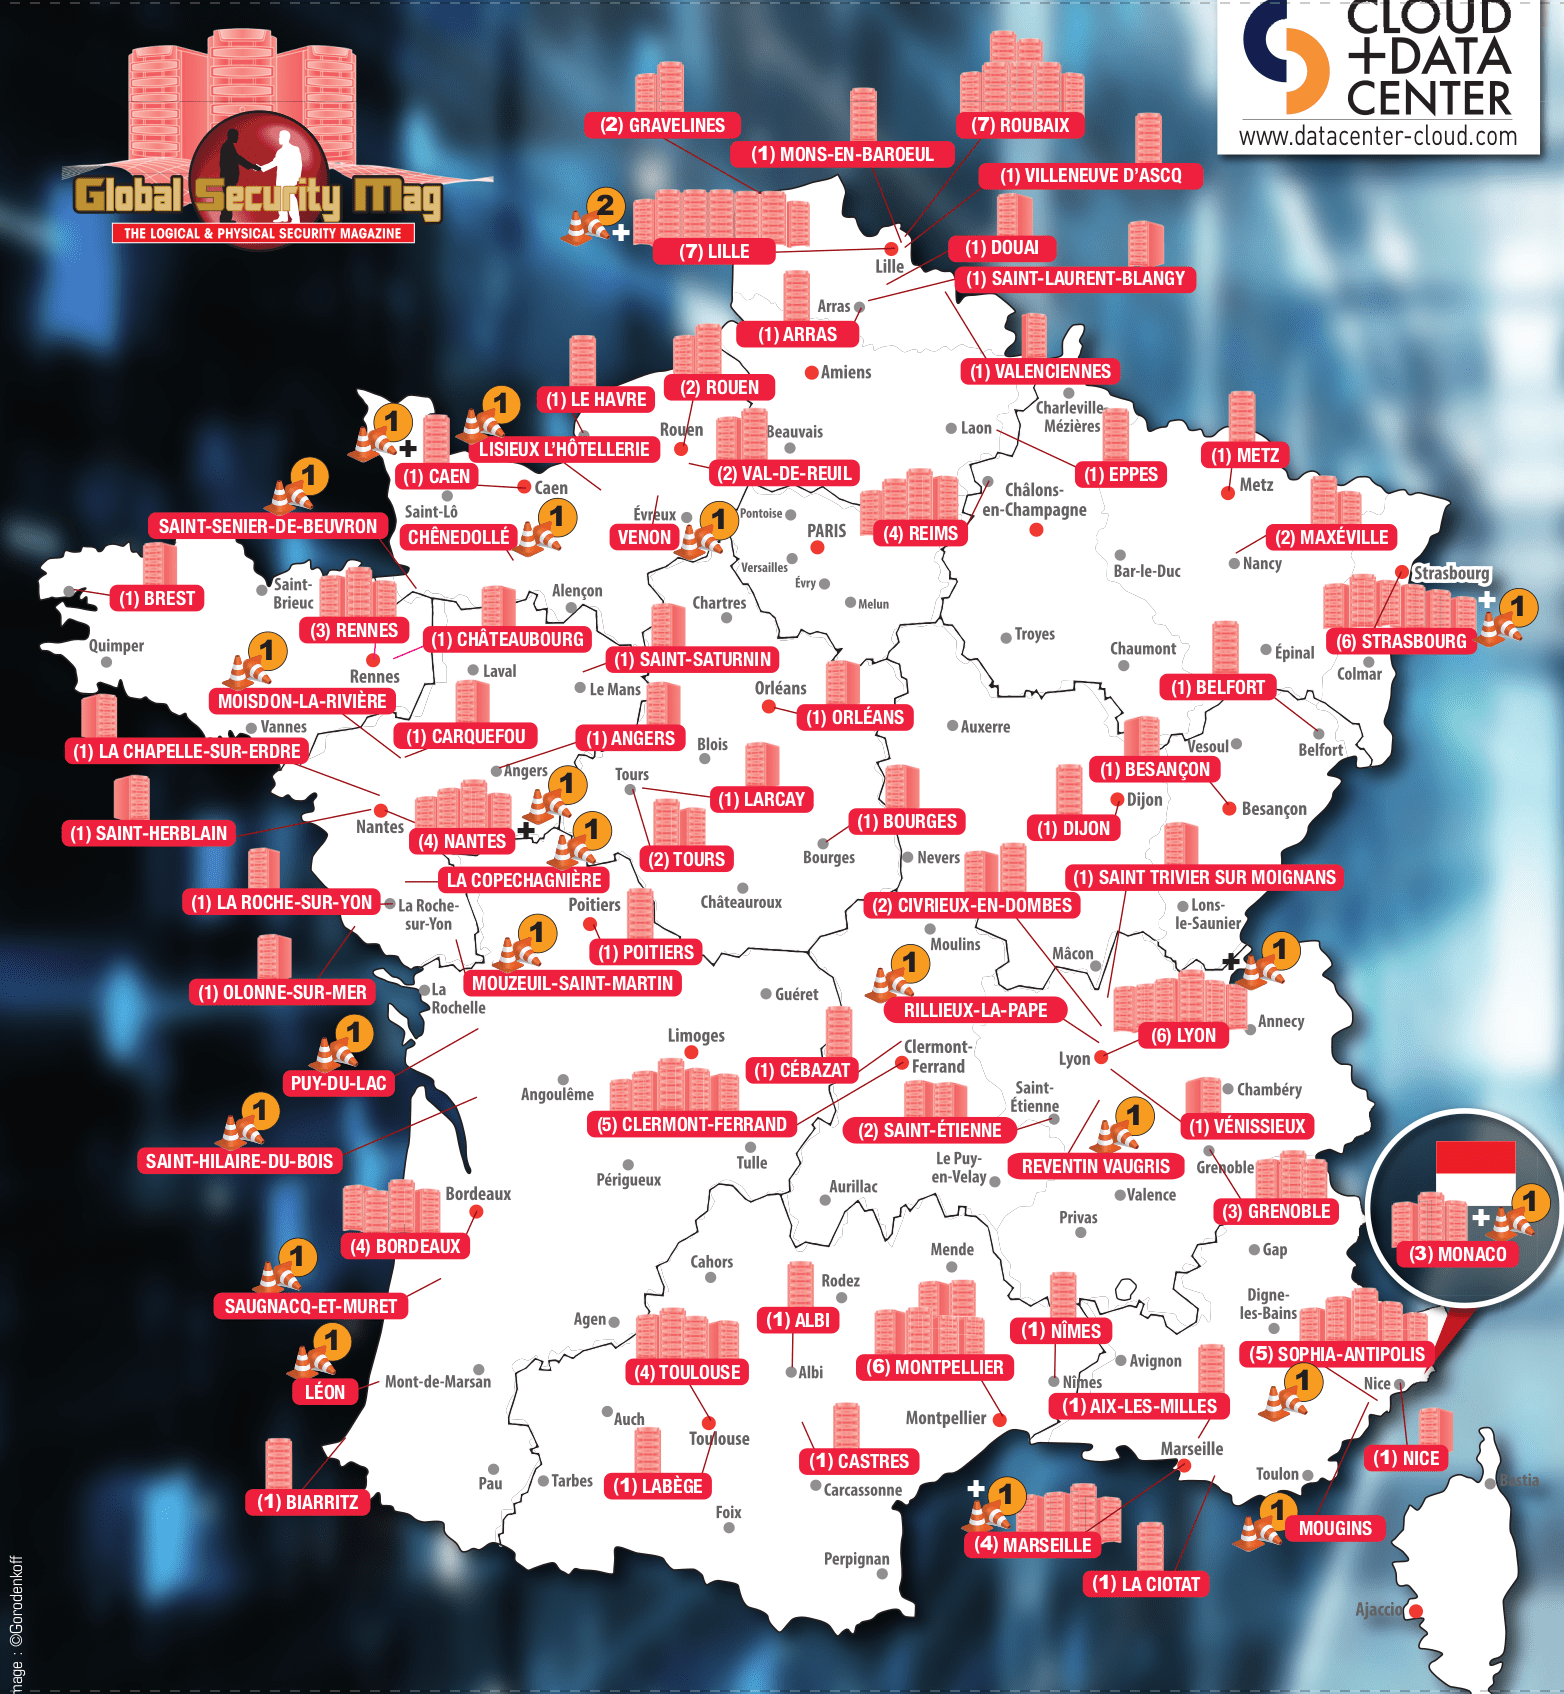
\includegraphics[width=\textwidth]{carte_data_center.png}
        \end{column}
        \begin{column}{0.5\textwidth}
            \begin{itemize}
                \item Plus de la moitié des \textit{data center} français sont en zone urbaine
                \item 3 \% de la consommation mondiale d'électricité
                \item Objectif : réduire leur consommation
            \end{itemize}
        \end{column}
    \end{columns}
\end{frame}

\begin{frame}
    \frametitle{Plan}
    \begin{enumerate}
        \item Modélisation d'un data center
        \item Grandeurs caractéristiques
        \item Puissance consommée
        \item Simulation d'un data center
        \item Répartition optimale avec l'algorithme du gradient
    \end{enumerate}
\end{frame}

\begin{frame}
    \frametitle{Modélisation d'un data center}
    \framesubtitle{Différents modèles}

    \begin{columns}
        \begin{column}{0.55\textwidth}
            \begin{itemize}
                \item Modèle non retenu : ordinateur de bureau
                \begin{itemize}
                    \item Dangereux (230 V)
                    \item Grande inertie thermique
                \end{itemize}
                \item Modèle retenu : Raspberry Pi
                \begin{itemize}
                    \item Peu dangereux
                    \item Réponse rapide aux perturbations
                \end{itemize}
            \end{itemize}
        \end{column}
        \begin{column}{0.45\textwidth}
            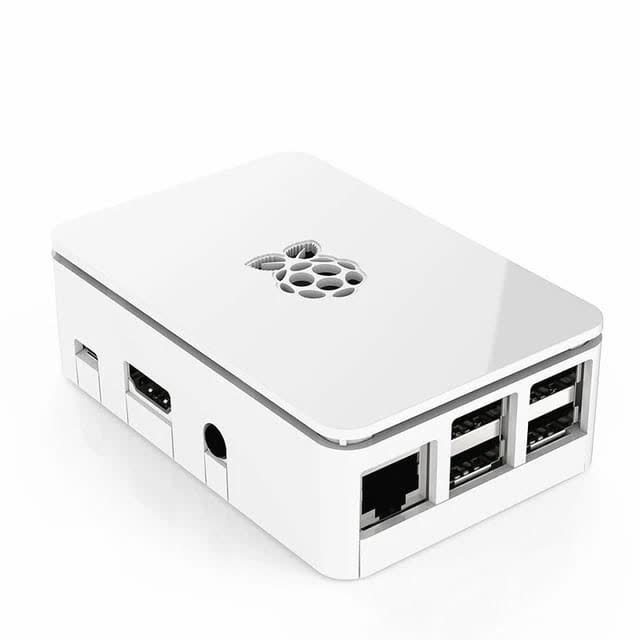
\includegraphics[width=0.8\textwidth]{raspberry_pi.jpg}
        \end{column}
    \end{columns}
\end{frame} % inconvénients des modèles non retenus

\begin{frame}
    \frametitle{Grandeurs caractéristiques}

    \begin{itemize}
        \item Masse volumique moyenne $\rho$ :
        \begin{itemize}
            \item Dimensions $\SI{85,60}{mm} \times \SI{53,98}{mm} \times \SI{17,00}{mm}$
            \item Masse $\SI{90,9}{g}$
            \item $\rho = \SI{1.16e3}{kg.m^{-3}}$
        \end{itemize}
        \item Capacité thermique massique moyenne $c$
        \item Conductivité thermique moyenne $\lambda$
    \end{itemize}
\end{frame}

\begin{frame}
    \frametitle{Grandeurs caractéristiques}
    \framesubtitle{Capacité thermique}

    \begin{center}
        \begin{tikzpicture}
            \node at (0, 0) {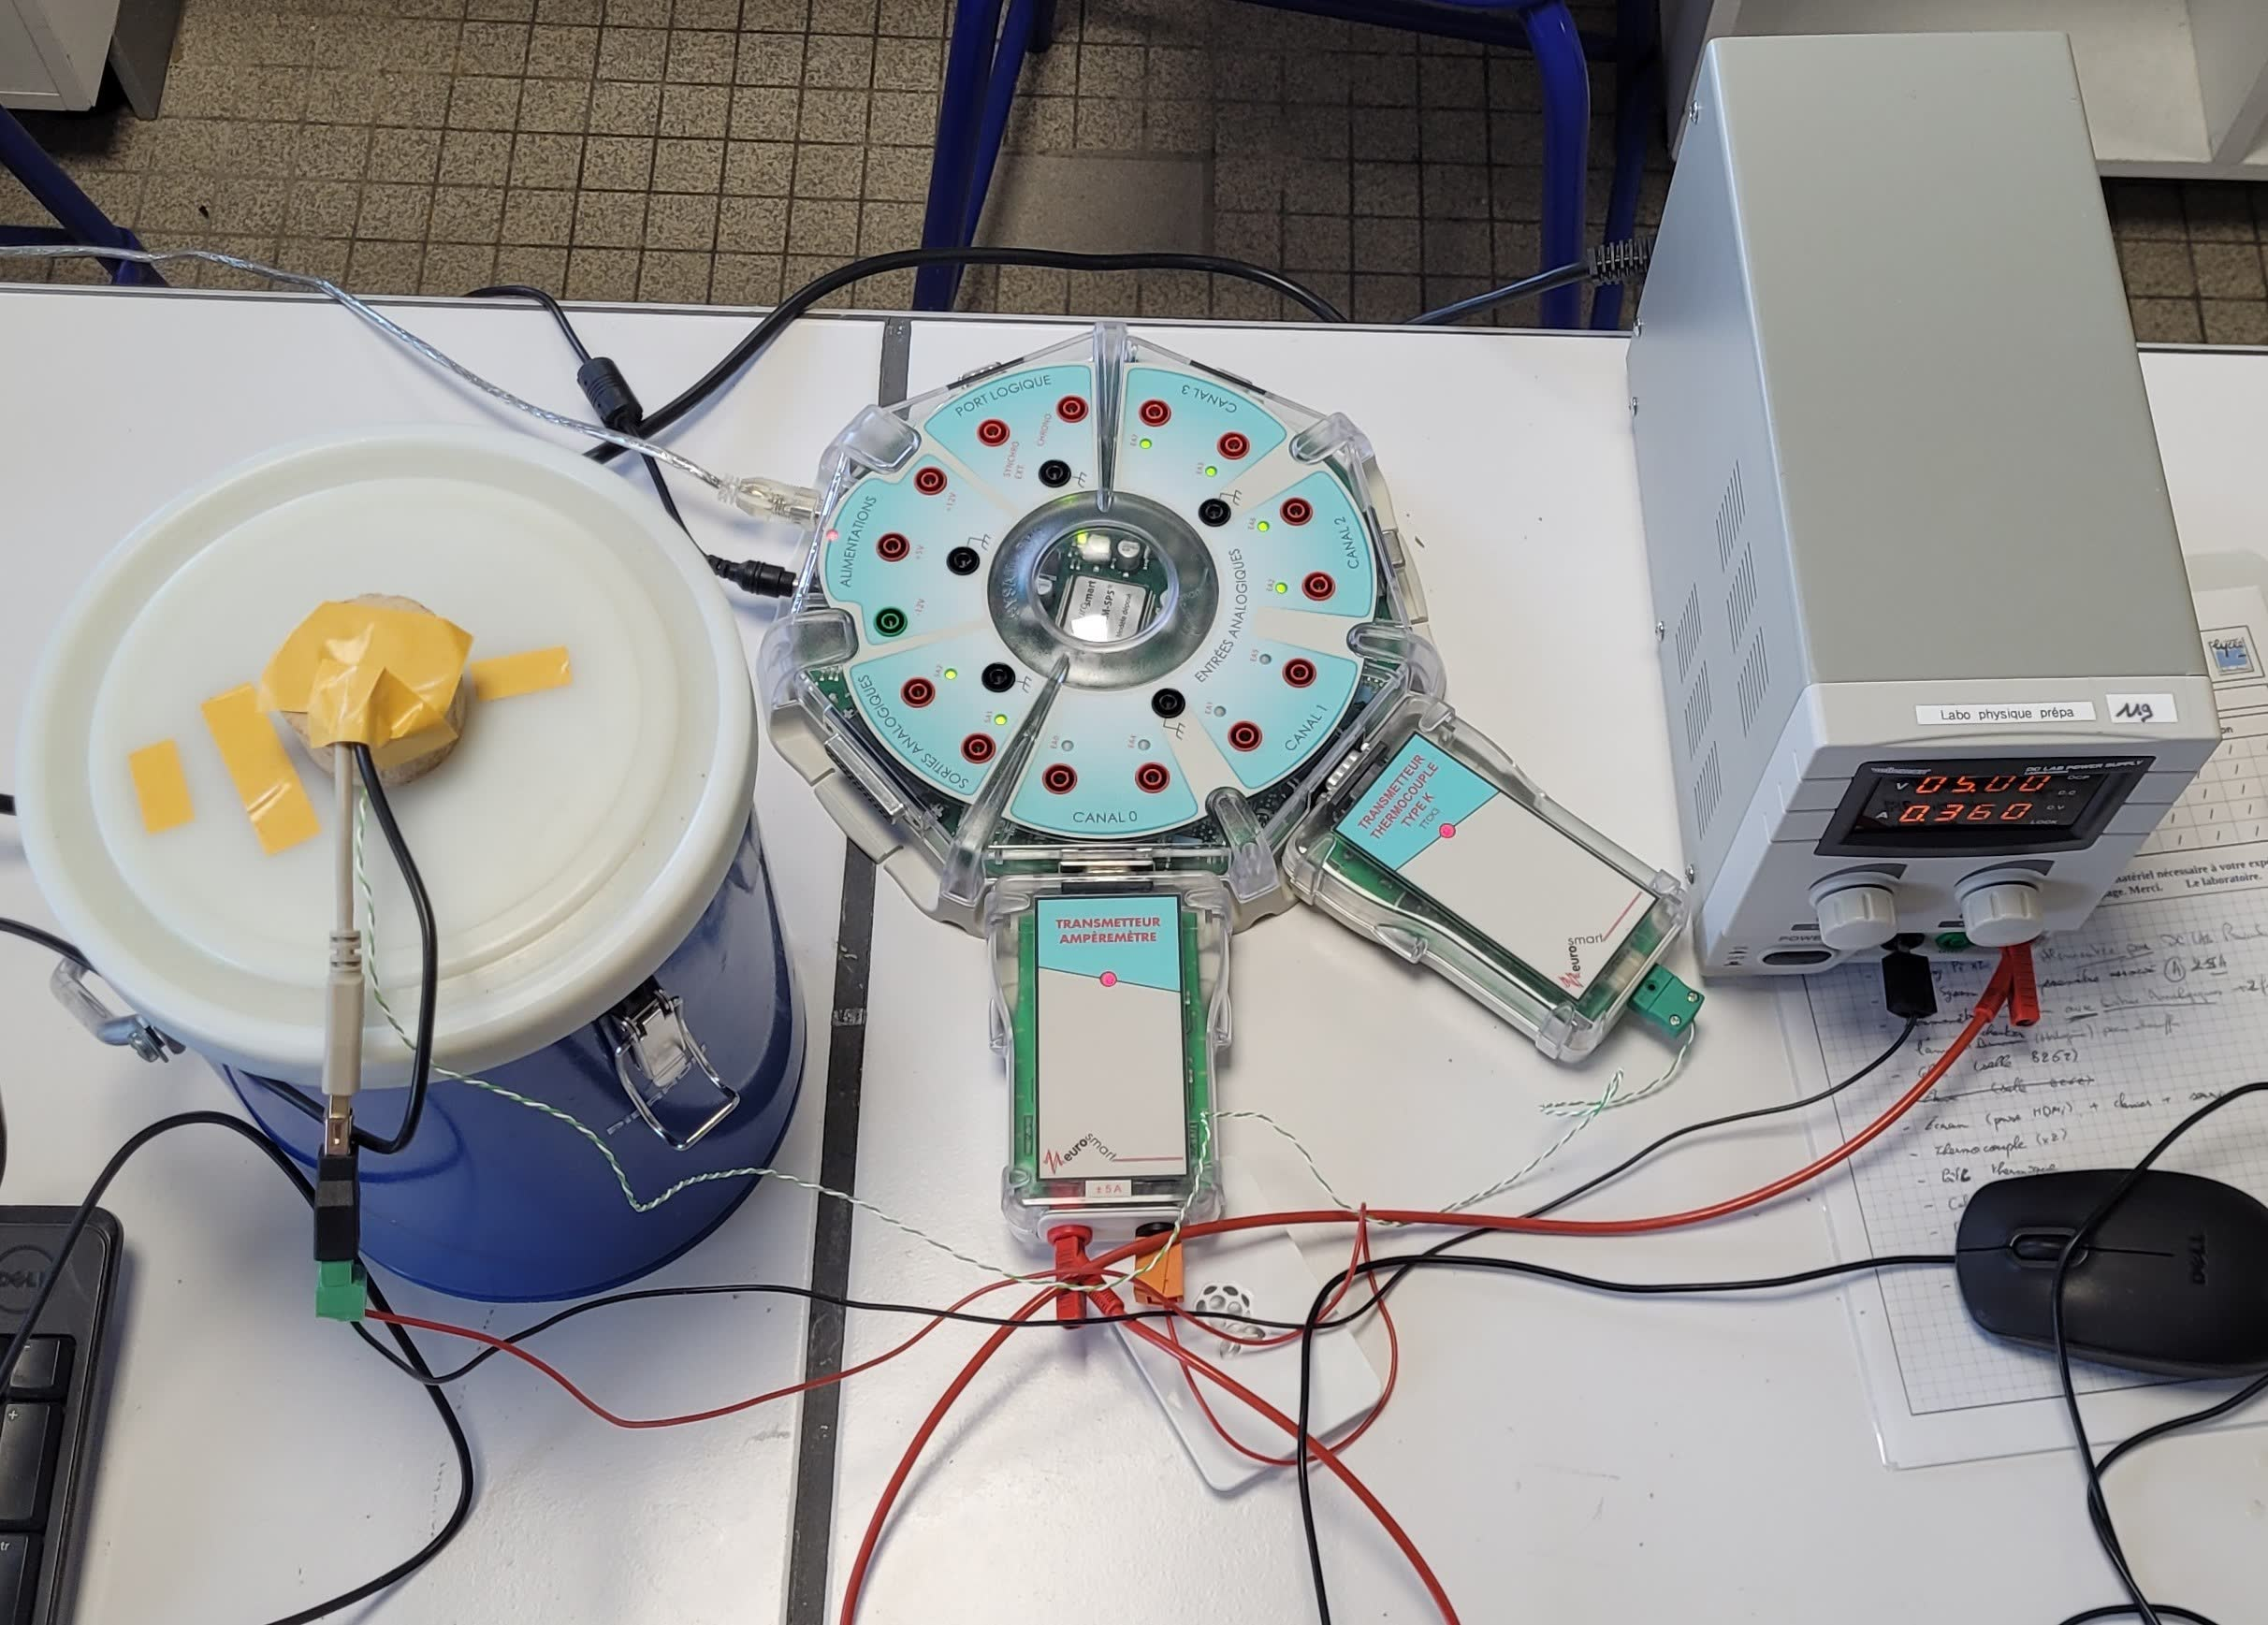
\includegraphics[width=0.7\textwidth]{tp-3.jpg}};
            \node at (-2, -4) {Calorimètre};
            \node at (6, 1.5) {Carte d'acquisition};
            \node at (6, 0) {Alimentation};
            \node at (2, -4) {Raspberry Pi (dans le calorimètre)};
            \node at (6, -4) {Ampèremètre};
            \node at (6, -2) {Thermocouple};

            \draw[->, line width=1mm] (-2, -3.5) -- (-2, 0); % Cal
            \draw[->, line width=1mm] (4.5, 1.5) -- (0, 0.5); % CS
            \draw[->, line width=1mm] (4.5, 0) -- (2.5, 0.5); % Ali
            \draw[->, line width=1mm] (0, -3.5) -- (-1.75, -0.5); % Rpi
            \draw[->, line width=1mm] (4.5, -2) -- (1.4, -0.4); % T
            \draw[->, line width=1mm] (6, -3.7) -- (0, -1); % A
        \end{tikzpicture}
    \end{center}
\end{frame}

\begin{frame}
    \frametitle{Grandeurs caractéristiques}
    \framesubtitle{Capacité thermique}

    \begin{columns}
        \begin{column}{0.55\textwidth}
            \begin{enumerate}
                \item[0.] Mesure de la masse en eau du calorimètre $m_\text{calo} = \SI{37}{g}$
                \item Avant calculs ($\SI{19,0}{\cel}$) intensité moyenne de 288 mA
                \item Lancement des calculs à $\SI{1}{min}$
                \item Fin des calculs à $\SI{6}{min}$. Pendant les calculs, on a
                \begin{itemize}
                    \item tension $\SI{5,0}{V}$
                    \item intensité moyenne 381 mA
                    \item travail électrique $\SI{612}{J}$
                \end{itemize}
                \item Thermalisation : sur les 100 dernières secondes, $\SI{20,6}{\cel}$
            \end{enumerate}
        \end{column}
        \vrule{}
        \begin{column}{0.45\textwidth}
            (1\ier{} principe) $\Delta U = W = C \Delta T$
            \begin{itemize}
                \item Capacité thermique $C = \SI{204}{J/K}$
                \item Capacité thermique massique $c = \SI{4,5}{kJ.K^{-1}.kg^{-1}}$
            \end{itemize}
        \end{column}
    \end{columns}
\end{frame}

\begin{frame}
    \frametitle{Grandeurs caractéristiques}
    \framesubtitle{Conductivité moyenne}

    Protocole
    \begin{enumerate}
        \item Plaque chauffante
        \item Mesure de la température aux deux extrémités
        \item Diffusion thermique : lien entre les températures et la conductivité
    \end{enumerate}
\end{frame}


\begin{frame}
    \frametitle{Grandeurs caractéristiques}
    \framesubtitle{Conductivité moyenne}
    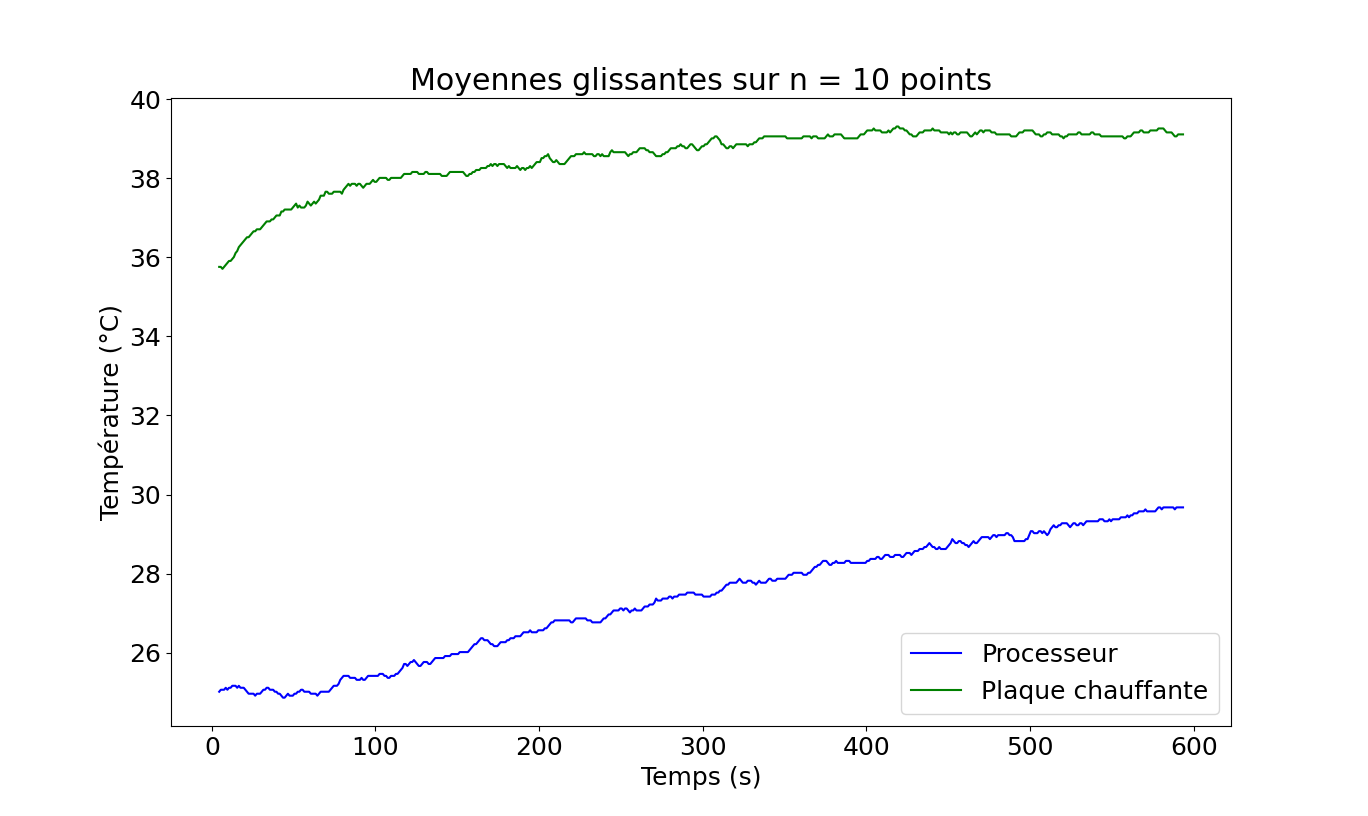
\includegraphics[width=\textwidth]{moyennes_glissantes.png}
    \begin{center}
        $\sigma = \frac{\Delta T}{\sqrt 3 \sqrt \text{pas}} = \SI{0,09}{\cel}$
    \end{center}
\end{frame}


\begin{frame}
    \frametitle{Grandeurs caractéristiques}
    \framesubtitle{Conductivité moyenne}
    On détermine $D$ grâce à l'équation de la diffusion
    $D = \SI{8.25e-8}{m^2/s}$ \hfill
    $\lambda = D \rho c = \SI{4.30e-4}{W.m^{-1}.K^{-1}}$

    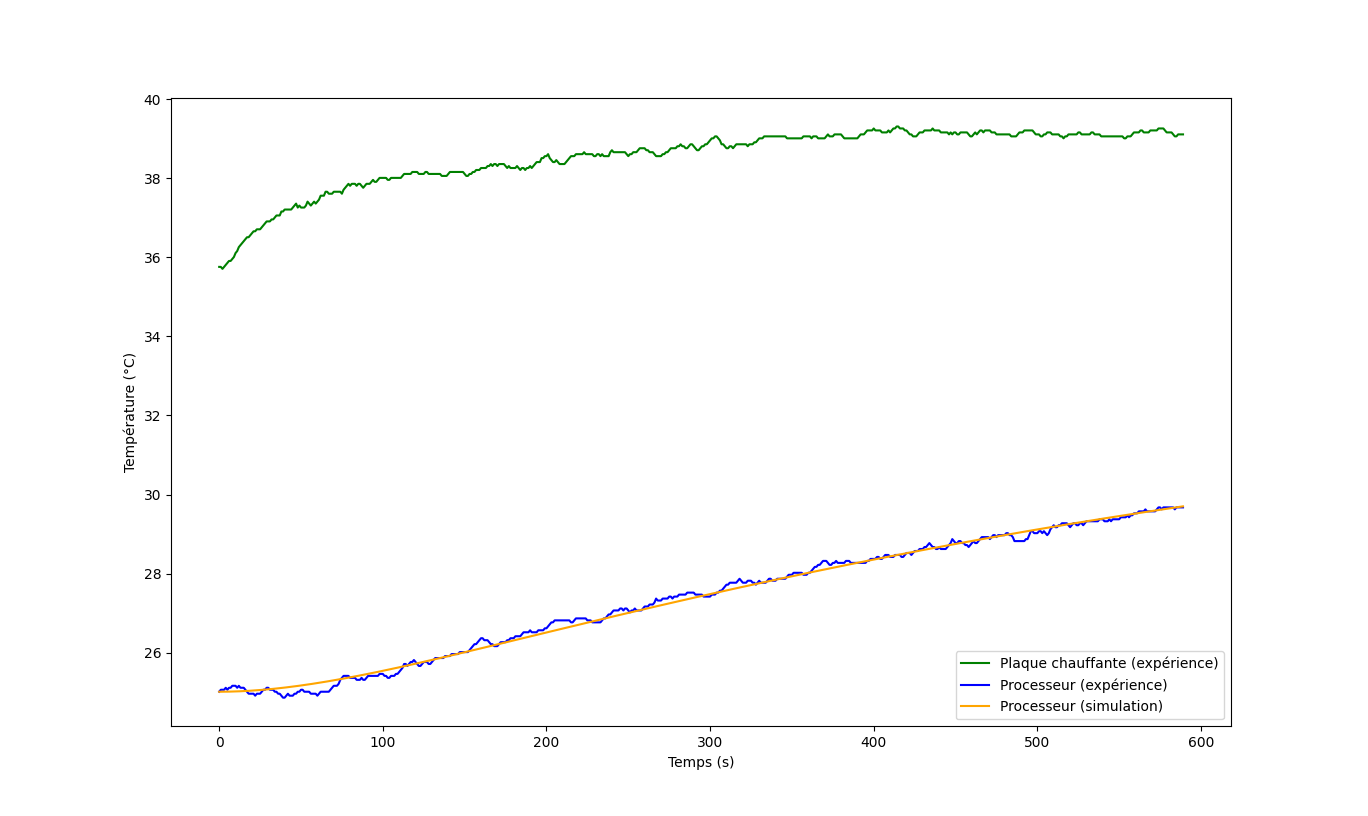
\includegraphics[width=\textwidth]{d_simulation.png}
\end{frame}

\begin{frame}
    \frametitle{Puissance consommée}

    \begin{enumerate}
        \item Définition de la quantité de calcul
        \item Mesure de la consommation du Raspberry Pi
        \item Régression linéaire
    \end{enumerate}
\end{frame}

\begin{frame}[fragile]
    \frametitle{Puissance consommée}
    \framesubtitle{Définition de la quantité de calcul}

    \begin{itemize}
        \item On note $K$ la quantité de calculs
        \item Unité standard : \textit{floating-point operation}
        \item Un calcul est une opération sur des flottants
        \item Défini à une constante additive près (au repos, $K = 0$)
        \begin{python}
def calculs(n):
    for _ in range(n):
        a, b = 60986.5150141834, 2831540.2372984355
        c = a ** (-b)
        \end{python}
    \end{itemize}
\end{frame}

\begin{frame}
    \frametitle{Puissance consommée}
    \framesubtitle{Dispositif expérimental}

    \begin{columns}
        \begin{column}{0.5\textwidth}
            \begin{enumerate}
                \item On modifie la température au processeur (glace, lampe de chantier)
                \item On impose la quantité de calculs
                \item On mesure l'intensité moyenne consommée
            \end{enumerate}
        \end{column}
        \begin{column}{0.5\textwidth}
            \begin{tikzpicture}
                \node at (0, 0) {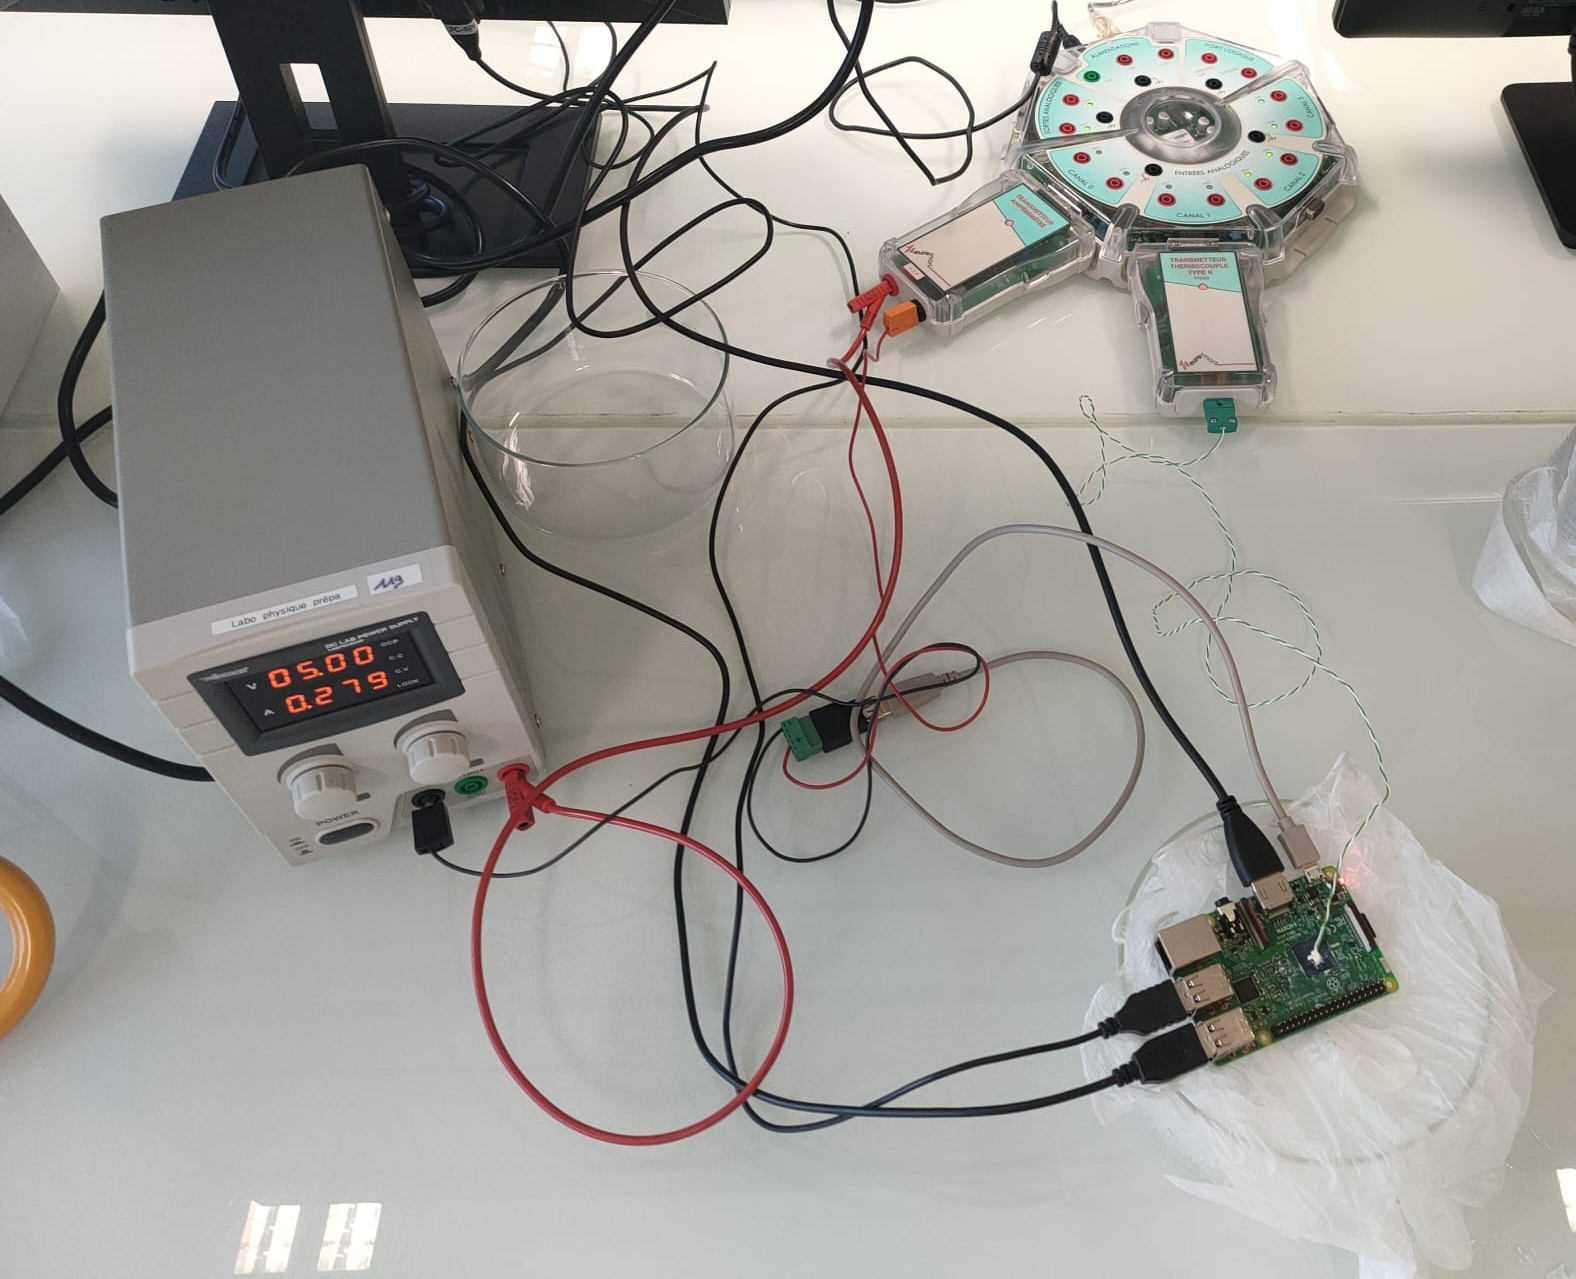
\includegraphics[width=\textwidth]{TP-2.3bis.jpg}};

                \node at (1, 3) {Raspberry Pi};
                \node at (1.5, -4) {Glace};
                \node at (-1, -4) {Lampe de chantier};

                \draw[->, line width=1mm] (1.5, -3.5) -- (1.9, -1.5); % gl
                \draw[->, line width=1mm] (1, 2.5) -- (1.9, -1); % rpi
                \draw[->, line width=1mm] (-1, -3.5) -- (-2.6, -1.2); % lampe
            \end{tikzpicture}
        \end{column}
    \end{columns}
\end{frame}

\begin{frame}
    \frametitle{Puissance consommée}
    \framesubtitle{Résultats expérimentaux}

    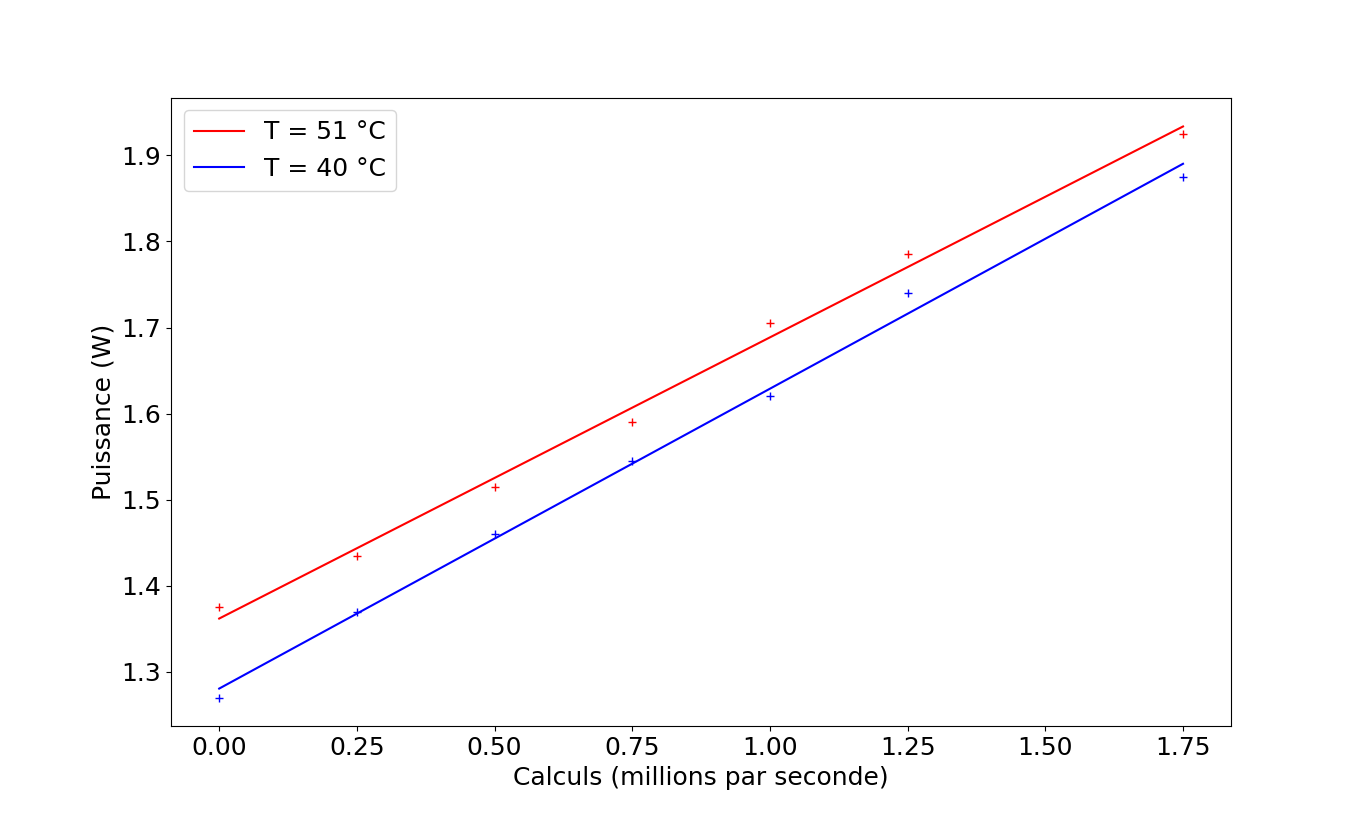
\includegraphics[width=0.9\textwidth]{difference_en_temperature.png}
    \begin{center}
        $P = a\times K + b(T)$
    \end{center}
\end{frame}

\begin{frame}
    \frametitle{Puissance consommée}
    \framesubtitle{Régression linéaire}

    \begin{itemize}
        \item Allure de plan
        $$P = a \times T + b \times K + c$$
        \item Régression linéaire avec \p{np.linalg.lstsq}
        \begin{itemize}
            \item $a = \SI{1.8e-3}{W/K}$
            \item $b = \SI{3.6e-1}{W/\text{millions de calculs par seconde}}$
            \item $c = \SI{0.94}{W}$
        \end{itemize}
    \end{itemize}
\end{frame}

\begin{frame}
    \frametitle{Puissance consommée}
    \framesubtitle{Régression linéaire}

    \begin{center}
        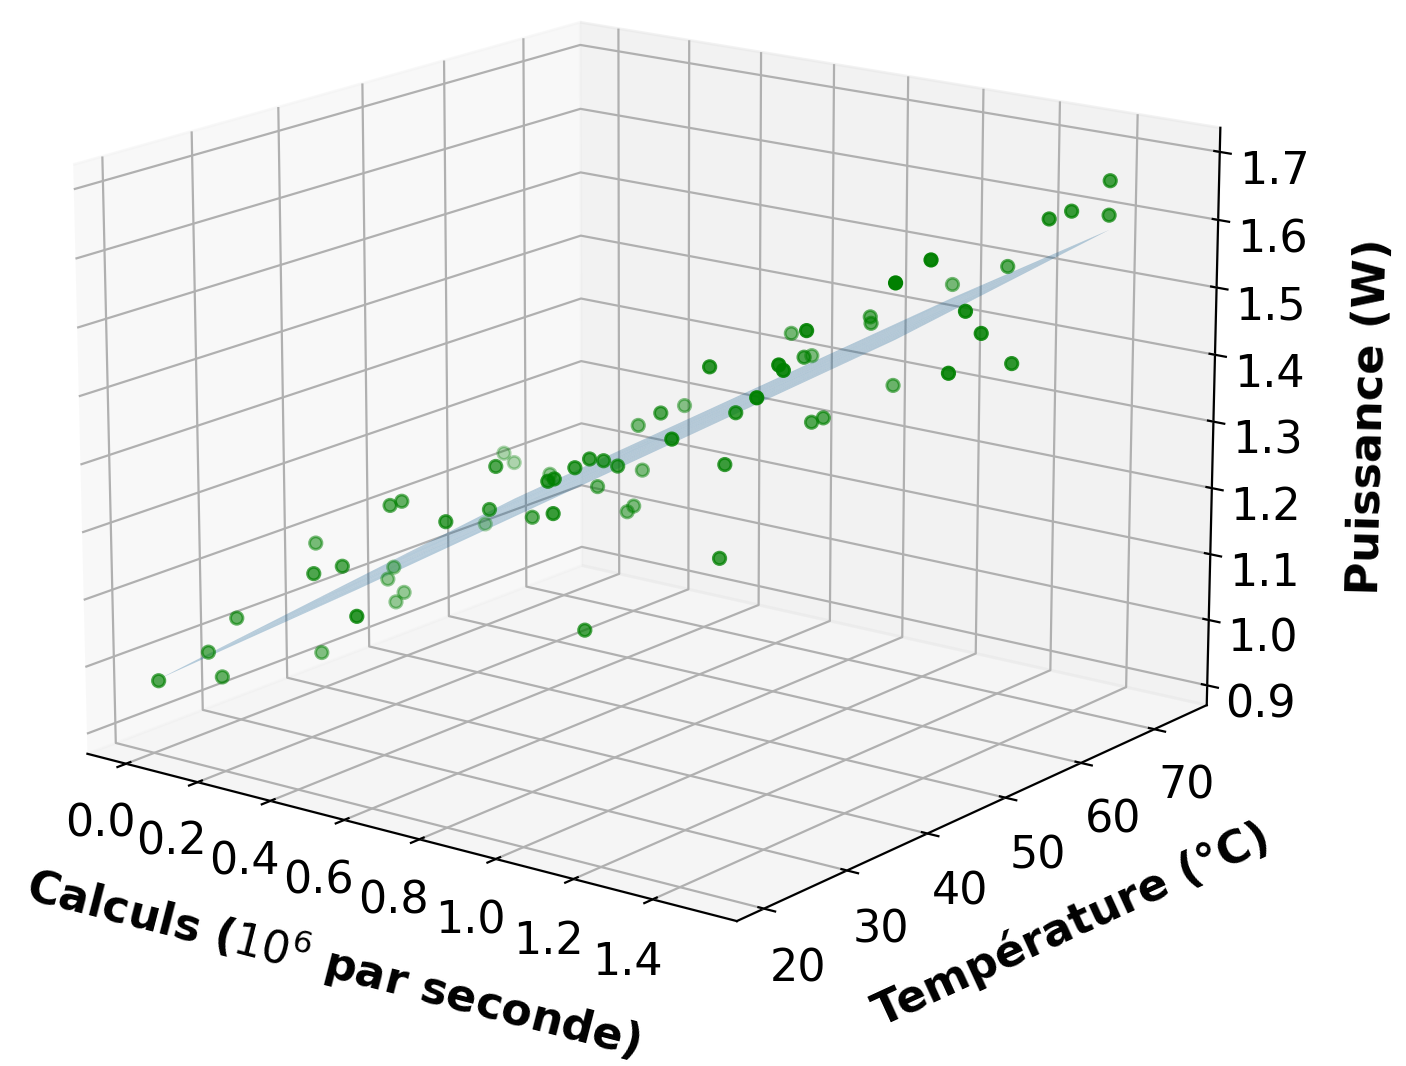
\includegraphics[width=0.7\textwidth]{regression_cube.png}

        Moyenne des écarts relatifs : 3 \%
    \end{center}
\end{frame}

\begin{frame}
    \frametitle{Simulation d'un data center}
    \framesubtitle{Hypothèses}

    \begin{itemize}
        \item Carcasse de l'ordinateur : pavé uniforme
        \item Source thermique : pavé centré sur la carcasse
        \begin{itemize}
            \item Puissance volumique uniforme
        \end{itemize}
        \item Air ambiant
        \begin{itemize}
            \item Pas de convection (seulement la diffusion)
        \end{itemize}
        \item Salle isolée
    \end{itemize}
\end{frame}

\begin{frame}[fragile]
    \frametitle{Simulation d'un data center}
    \framesubtitle{Principe de l'aglorithme}

    \begin{itemize}
        \item Temps et espace (1D) discrétisés
        \item Température : tableau \p{numpy} \p{T[x, t]}
        \item Équation aux dérivées partielles
            $$\pdv{T}{t} = D(x) \pdv[2]{T}{x} + P_c(x) \quad \text{où} \quad P_c(x) = \frac{P_v}{\rho c}$$
        \item Traduction informatique
        \begin{python}
T[xi, ti+1] = T[xi, ti] + (t_e / (x_e**2)) * D(xi)
    (T[xi+1, ti] - T[xi, ti] + T[xi-1, ti])
    + P_c(xi) * t_e
        \end{python}
    \end{itemize}
\end{frame}

\begin{frame}
    \frametitle{Répartition optimale}
    \framesubtitle{Ordinateurs multiples et dépendances}

    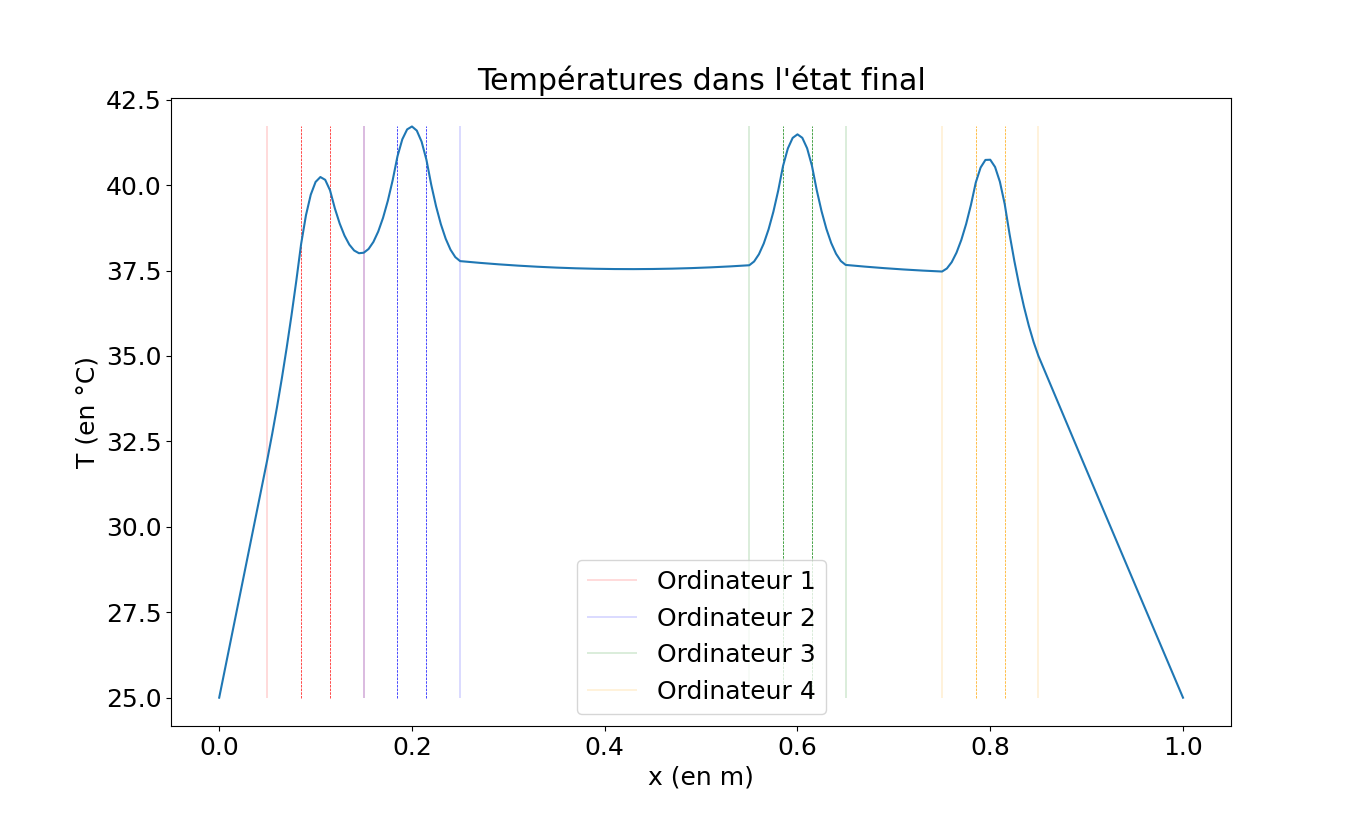
\includegraphics[width=\textwidth]{positions.png}
\end{frame}

\begin{frame}
    \frametitle{Répartition optimale}
    \framesubtitle{Algorithme du gradient}

    Pour trouver un minimum d'une fonction $f$ :
    \begin{itemize}
        \item Calcul du gradient au point $M$, $\grad f (M)$
        \item Test d'arrêt : fin si $||\grad f (M)|| < \varepsilon$
        \item Nouveau point $M \leftarrow M - \alpha \times \grad f (M)$
    \end{itemize}

    Coordonnées réduites : $\frac{x_i}{L}$ et $\frac{K_i}{K}$ pour avoir $f : [0, 1]^{2n} \rightarrow \mathbb{R}$
\end{frame}

\begin{frame}
    \frametitle{Répartition optimale}
    \framesubtitle{Résultats qualitatifs}

    \begin{itemize}
        \item Éviter de tout concentrer au centre
        \item Donner autant de calculs à chaque groupe d'ordinateurs
        \item Dans chaque groupe, l'ordinateur le plus proche du mur a plus de calculs
    \end{itemize}
\end{frame}

\begin{frame}
    \frametitle{Répartition optimale}
    \framesubtitle{Configurations optimales}

    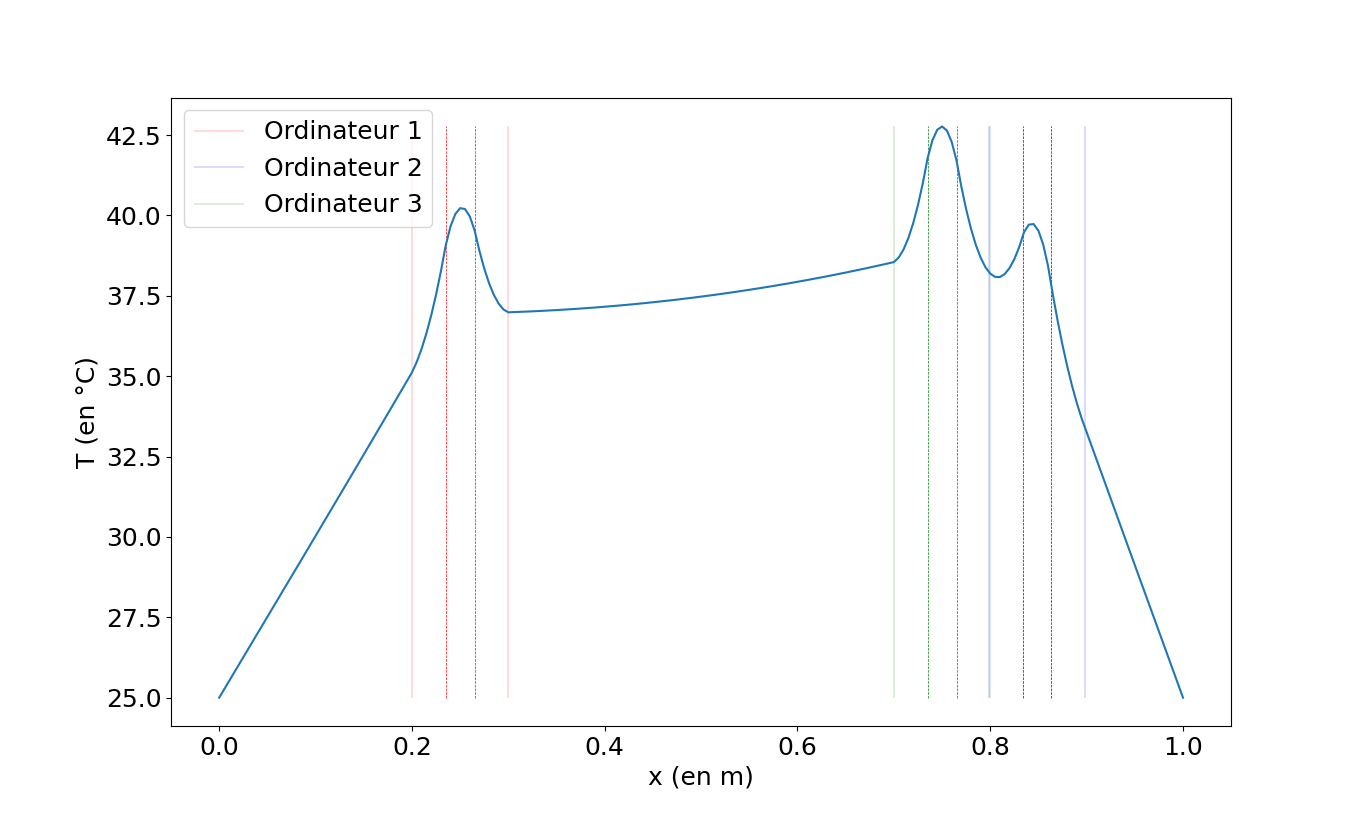
\includegraphics[width=\textwidth]{min_position.png}

    \begin{center}
        Après $\SI{12}{h}$ de calculs
    \end{center}
\end{frame}

\begin{frame}
    \frametitle{Répartition optimale}
    \framesubtitle{Configurations optimales}

    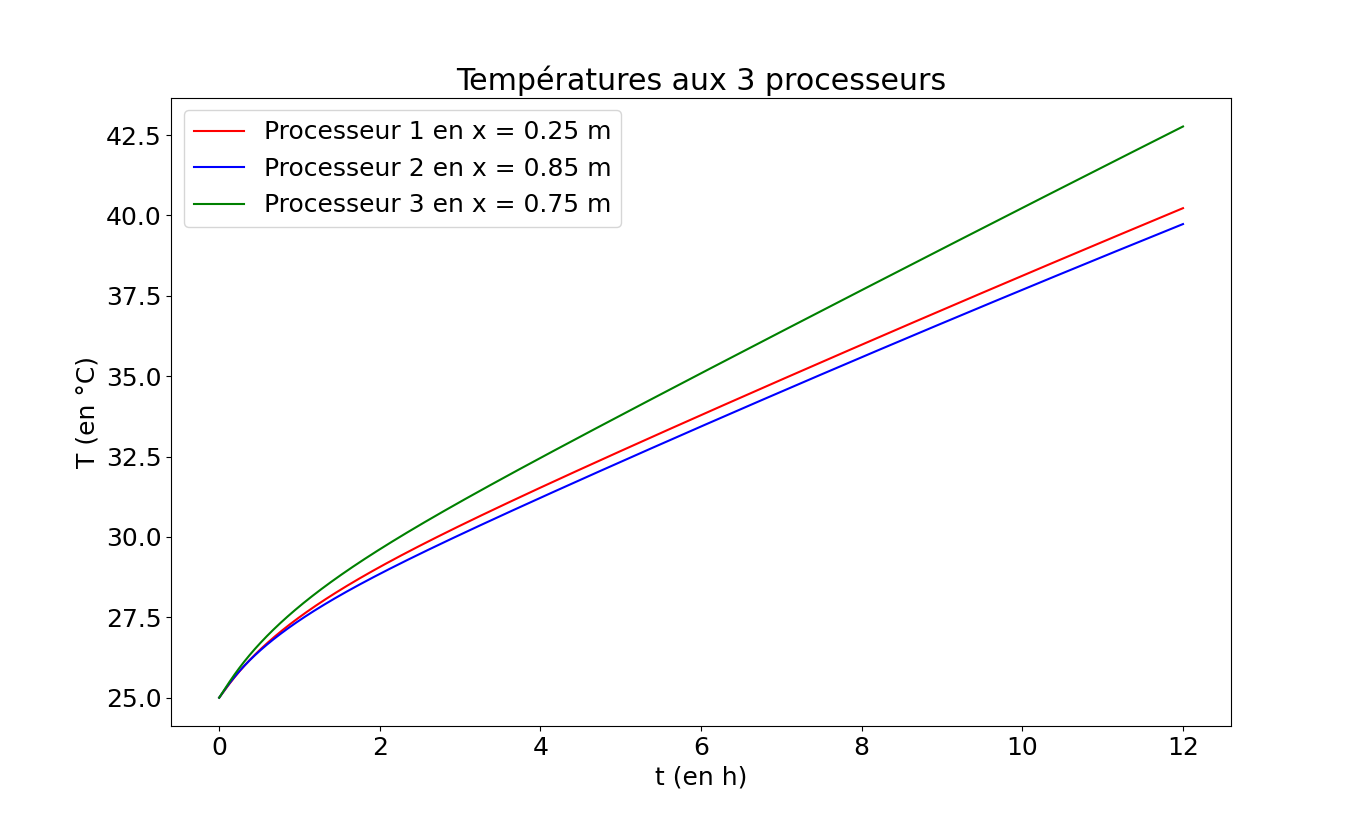
\includegraphics[width=\textwidth]{min_temperature.png}
\end{frame}

\begin{frame}
    \frametitle{Répartition optimale}
    \framesubtitle{Configurations optimales}

    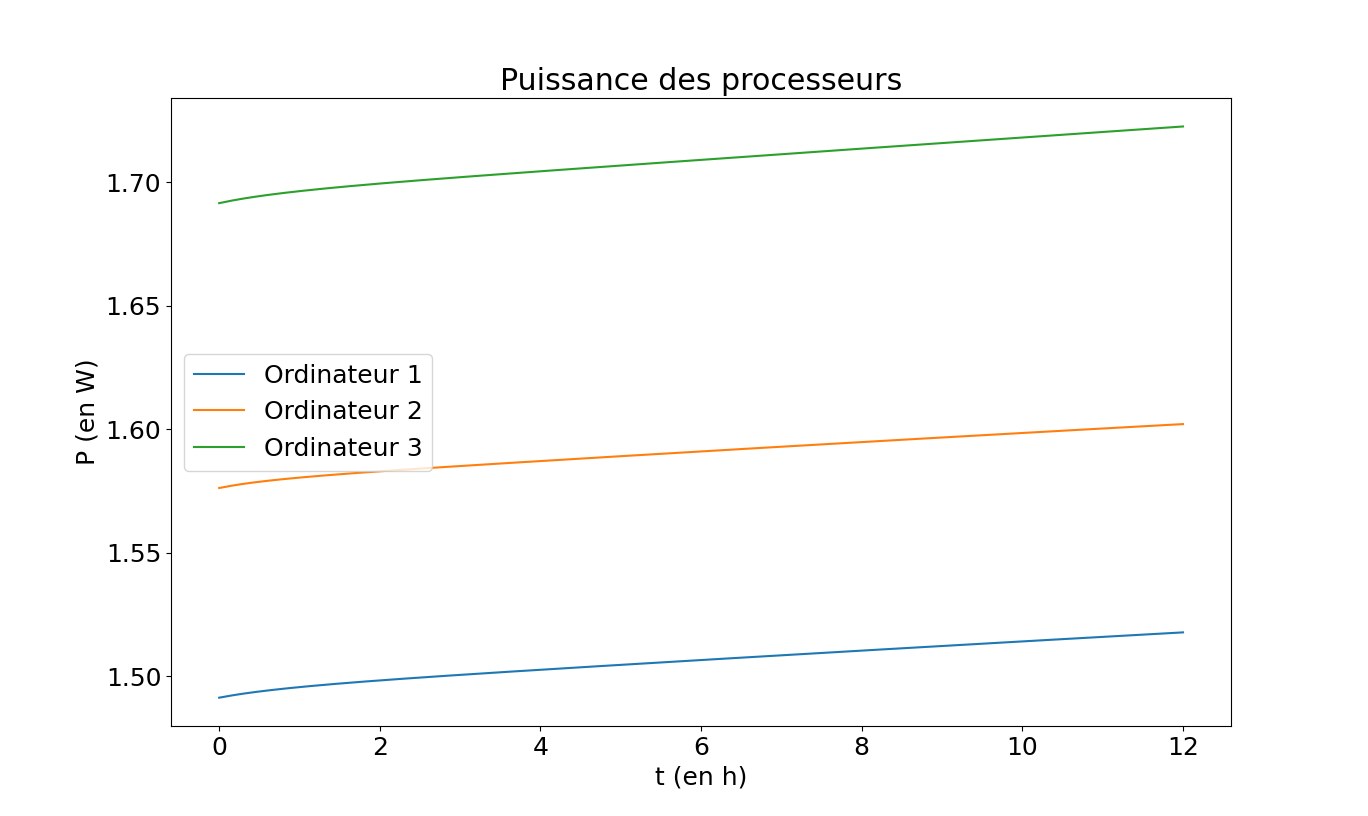
\includegraphics[width=\textwidth]{min_puissance.png}

    \begin{center}
        Énergie consommée en $\SI{12}{h}$ : $\SI{20,8}{kJ}$ soit $\SI{0.06}{kWh}$
    \end{center}
\end{frame}

\begin{frame}[plain, noframenumbering]
    \frametitle{Conductivité moyenne}
    \framesubtitle{Données brutes}

    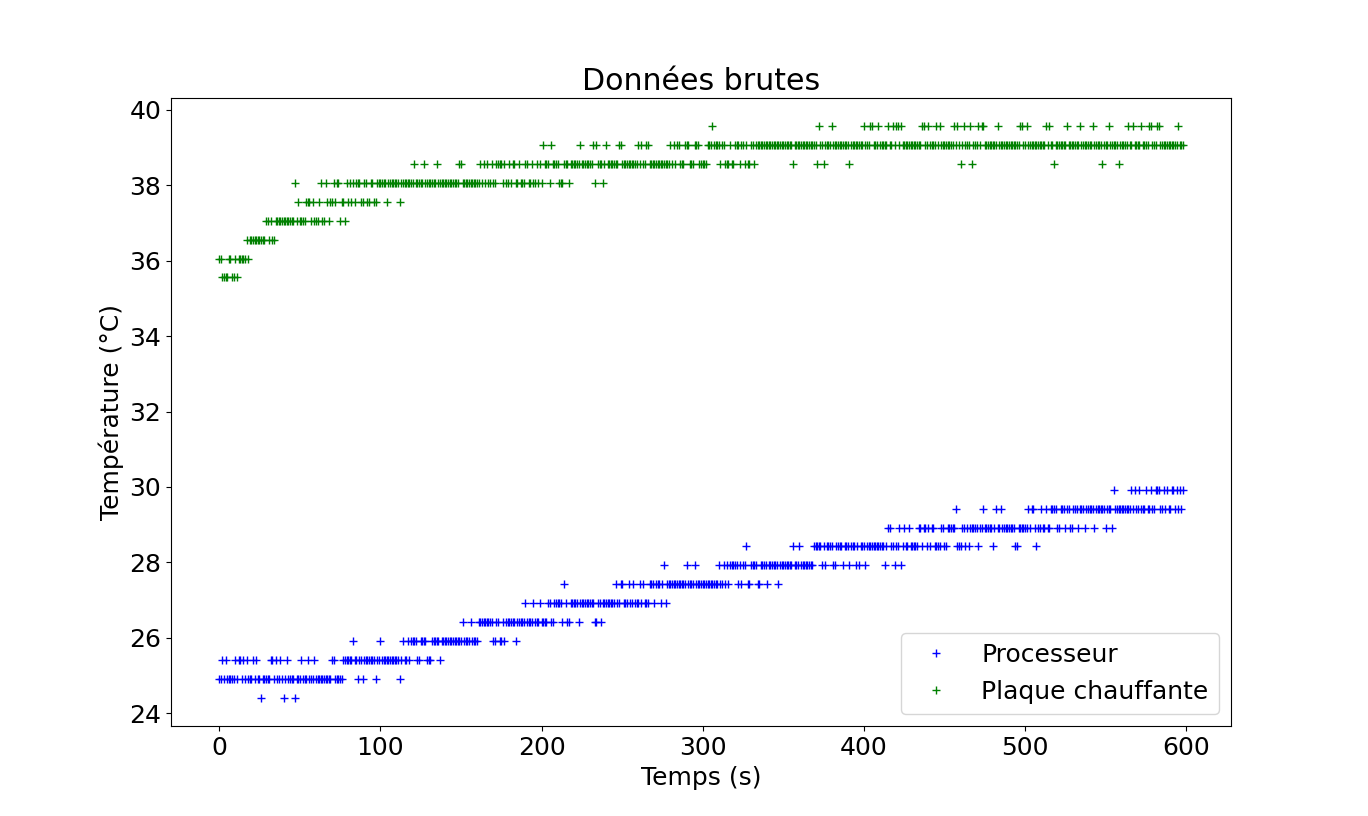
\includegraphics[width=\textwidth]{donnees_brutes.png}
\end{frame}

\begin{frame}[plain, noframenumbering]
    \frametitle{Conductivité moyenne}
    \framesubtitle{Écart-type par Monte-Carlo}

    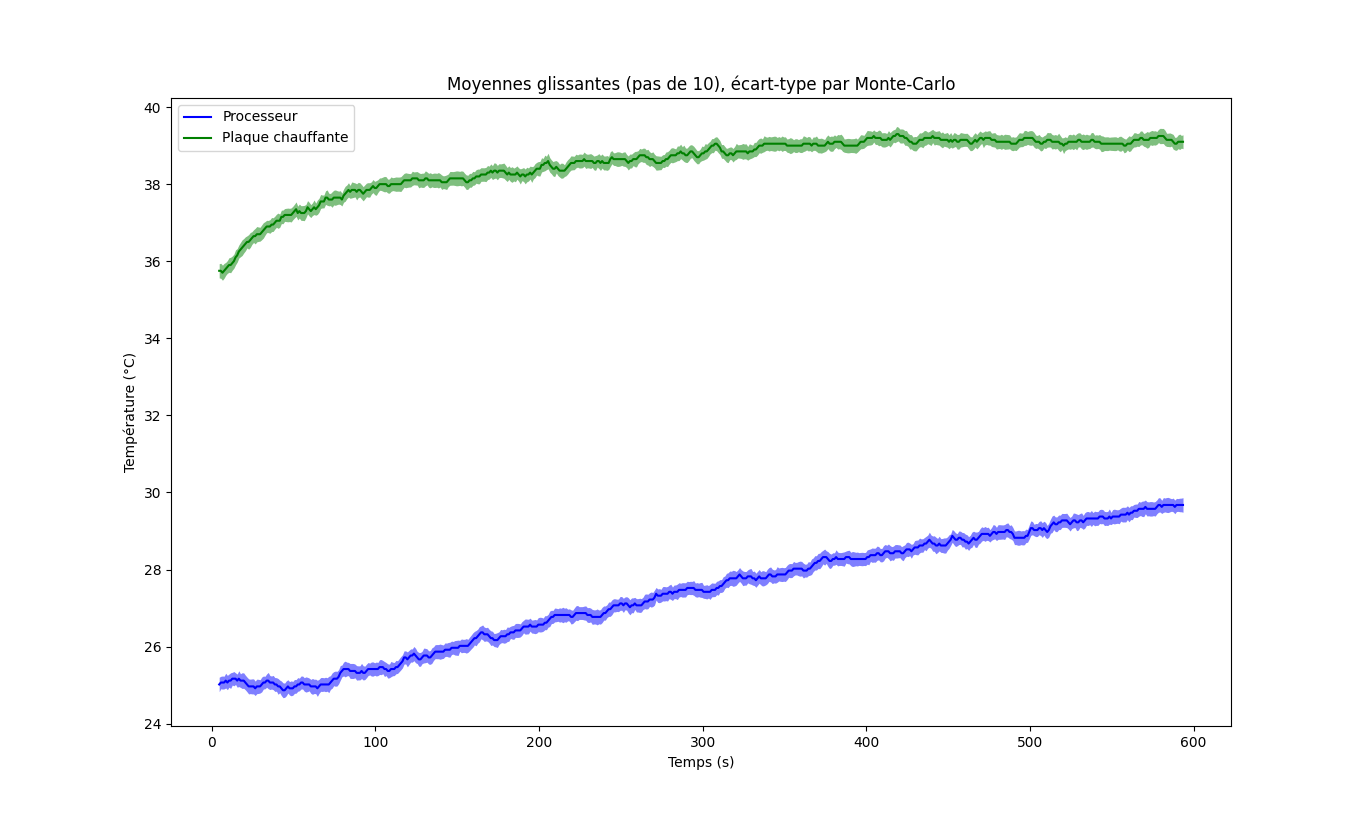
\includegraphics[width=\textwidth]{moyennes_glissantes_monte_carlo.png}
\end{frame}
%=====================================================
%=====================================================
%=====================================================

\end{document}
